\chapter{Related Work}\label{cha:related}

\section{Convergence theory for overparameterized neural networks}
\label{sec:related-convergence}

A central question in the theory of neural-network training is why
gradient-based optimization can reach small or even zero training loss despite
the non-convexity of the parameter-space objective. A major line of work
addresses this question in overparameterized regimes by proving that gradient
descent or stochastic gradient descent can converge to global minimizers when
the network is sufficiently wide
\citep{du2019gradient,allen2019convergence,
	arora2019finegrainedanalysisoptimizationgeneralization}.
A closely related viewpoint shows that, in large-width regimes, networks can
remain close to their linearization around initialization, so that the tangent
kernel stays stable during training
\citep{jacot2018ntk,lee2020wide}. In this regime, the training dynamics can be
analyzed as kernel dynamics rather than as a general non-convex optimization
problem.

\paragraph{Infinite-width NTK dynamics.}
The Neural Tangent Kernel framework of \citet{jacot2018ntk} gives one of the
cleanest such descriptions. In the infinite-width limit, the NTK converges to a
deterministic limiting kernel and remains constant during training
\citep{jacot2018ntk,lee2020wide}. For the squared loss, this reduces the
evolution of the network function to a linear differential equation in function
space. Convergence is then controlled by the spectrum of the limiting kernel,
and in particular by its positive-definiteness on the training data
\citep{jacot2018ntk}. This provides a direct link between training dynamics,
kernel eigenvalues, and convergence rates.

\paragraph{Finite-width global convergence in the overparameterized regime.}
A related line of work proves that sufficiently wide but finite networks can be
trained to global minima by gradient descent or stochastic gradient descent. For
example, \citet{du2019gradient} show that gradient descent achieves zero
training loss for overparameterized deep networks by controlling the stability
of the Gram matrix induced by the network. Similarly,
\citet{allen2019convergence} prove convergence of gradient-based optimization
for sufficiently overparameterized deep networks, with width polynomial in the
number of samples and depth under suitable assumptions on the data. These
results show that overparameterization can make the local geometry around
random initialization regular enough for global convergence, even though the
original objective is non-convex.

\paragraph{Optimization and generalization in the NTK regime.}
Other works refine this kernel-based view by studying both optimization and
generalization. \citet{arora2019finegrainedanalysisoptimizationgeneralization}
analyze overparameterized two-layer ReLU networks through a kernel perspective,
showing that the network behaves similarly to kernel regression in the
overparameterized regime. Such results help explain why training can converge
rapidly in wide networks, but they also emphasize that the conclusions rely on
regimes where the tangent features do not move too far from initialization
\citep{arora2019finegrainedanalysisoptimizationgeneralization,lee2020wide}.

\begin{revblock}
	\paragraph{Limits of the fixed-kernel picture.}
	The NTK regime gives a tractable description of training, but it is also a
	restrictive approximation. In the infinite-width limit with fixed depth, the
	tangent kernel becomes deterministic and stays constant during training, so
	learning is described by a fixed feature map
	\citep{jacot2018ntk,lee2020wide}. At finite width, this picture can fail in two
	ways: the tangent kernel is random at initialization, and it can also change
	during training.

	\citet{haninNica2019finite} show that finite depth and finite width can produce
	non-negligible fluctuations in the NTK at initialization. In particular, they
	find that the variance of the NTK depends on the ratio between depth and width,
	so the infinite-width deterministic-kernel picture is not automatically
	accurate when depth and width grow together. They also show that, in such
	regimes, the NTK can have non-trivial evolution during training. In other
	words, the tangent kernel itself can move during training, not merely fluctuate
	around its initial value. This suggests that finite networks need not behave
	exactly like their frozen infinite-width kernel counterparts.

	\citet{bordelon2023dynamicsfinitewidthkernel} study the dynamics of finite-width
	kernel and prediction fluctuations during training. Their analysis separates the
	lazy regime, where the kernel is random but essentially static, from feature
	learning regimes, where kernel fluctuations and prediction fluctuations evolve
	together. This is relevant here because the evolving tangent kernel can change
	not only the size of the learning rates, but also the directions in function
	space along which learning takes place.

	Finally,
	\citet{vyas2022limitationsntkunderstandinggeneralization} give empirical
	evidence that NTK models can fail to reproduce the generalization behavior of
	finite neural networks on realistic tasks. They also find that the empirical NTK
	can continue to evolve during much of training, rather than stabilizing after a
	short initial period. This reinforces the point that the fixed-kernel NTK should
	be treated as a useful reference model, not as a complete description of finite
	network training.

	These works motivate the comparison made in this thesis. We use the continuum
	infinite-width NTK as the reference operator, but we also study the frozen
	finite-width tangent kernel at initialization and the evolving finite-width
	tangent kernel during training.
\end{revblock}


\section{Spectral bias}\label{sec:spectral-bias}

A striking and widely reported phenomenon in neural network training is that
gradient-based optimization does not fit all components of a target function at
the same rate. Instead, networks tend to learn simple, slowly varying structure
first and refine fine-scale or highly oscillatory structure later. This
preference is commonly referred to as \emph{spectral bias} or the
\emph{frequency principle}. In its classical formulation, spectral bias asserts
that, when a target function is decomposed into Fourier modes, lower-frequency
components are learned earlier and at a faster rate than higher-frequency
components
\citep{rahaman2019spectralbiasneuralnetworks,xu2019training,zhi2020frequency}.

In this section, we briefly review empirical evidence for spectral bias and
summarize theoretical viewpoints that relate it to the spectrum of the operator
governing training dynamics in the kernel (NTK) regime. We also highlight
extensions that study how the phenomenon depends on the input distribution and
how it manifests outside the training set.

\subsection{Empirical evidence and the frequency principle}

A standard way to empirically probe spectral bias is to choose a target with a
controlled frequency decomposition and to track the frequency content of the
network's prediction $f_t$ during training.

\paragraph{Synthetic Fourier regression.}
A canonical experiment is 1D regression on a target constructed as a sum of
sinusoids,
\[
	y(z)=\sum_{i=1}^r A_i \sin(2\pi k_i z + \phi_i),
	\qquad z\in[0,1],
\]
and monitoring the discrete Fourier spectrum of the learned predictor as a
function of training time. \citet{rahaman2019spectralbiasneuralnetworks} report
that, for deep ReLU networks trained by (full-batch) gradient descent, Fourier
coefficients at smaller frequencies $k_i$ grow substantially earlier than those
at larger $k_i$, even when the amplitudes are matched or when high-frequency
components have larger amplitude \citep{rahaman2019spectralbiasneuralnetworks}.
This ``frequency-dependent learning speed'' is one of the most direct empirical
signatures of spectral bias.

Related work under the name \emph{frequency principle} reports a similar
ordering in the frequency domain: lower frequencies are fitted earlier during
training, while higher frequencies are fitted later
\citep{xu2019training,zhi2020frequency}. These observations support the view
that spectral bias is a statement about the training dynamics, not just about
which functions can be represented by the network.

\paragraph{Robustness and perturbation tests.}
A complementary protocol is to train to near-zero training error and then apply
random perturbations in parameter space, comparing how the Fourier spectrum of
the realized function changes. \citet{rahaman2019spectralbiasneuralnetworks}
observe that lower-frequency components of the learned function are
substantially more robust to such perturbations than higher-frequency
components, suggesting that the network parameterization itself represents low
frequencies in a more stable manner \citep{rahaman2019spectralbiasneuralnetworks}.

\begin{revblock}
	This matters because the perturbations are applied around the minimizer reached by training. If the
	low-frequency part changes little under such local perturbations, then small
	movements in parameter space do not strongly affect those components of the
	learned function, while higher-frequency components are more sensitive to the
	same perturbations. This provides further evidence that gradient-based training
	learns low-frequency components in a more stable way than high-frequency
	components, not only that it learns them earlier.
\end{revblock}

\begin{revblock}
	\subsection{Theoretical explanations in the NTK regime}

	The NTK viewpoint connects convergence theory to spectral bias; see Section~
	\ref{sec:ntk-spectral-dynamics}. In the fixed-kernel regime, the residual
	evolves under a kernel operator. When this operator is diagonalized into
	eigenfunctions, each residual component decays at a rate determined by the
	corresponding eigenvalue. \citet{cao2020understandingspectralbiasdeep} make
	this connection explicit for the NTK regime by showing that components aligned
	with larger eigenvalues are learned faster. Spectral bias can therefore be
	viewed as a refined convergence statement, where some directions in function
	space decay faster than others.

	This operator viewpoint becomes a frequency statement in settings with
	enough symmetry. \citet{basri2019convergence},
	\citet{bietti2019inductivebiasneuraltangent}, and
	\citet{cao2020understandingspectralbiasdeep} analyze settings in which
	one-hidden-layer ReLU networks and related NTK models are considered on the
	circle \(S^1\) or sphere \(S^{d-1}\), with isotropic initialization and uniform
	input distribution. In these settings, the limiting NTK is rotation-invariant,
	and the associated operator is diagonal in a harmonic basis.\footnote{A harmonic
		basis is an orthogonal decomposition of \(L^2\) into eigenspaces of the
		Laplace--Beltrami operator. See: \href{https://en.wikipedia.org/wiki/Spherical_harmonics}
		{https://en.wikipedia.org/wiki/Spherical\_harmonics}} On
	\(S^1\), the eigenfunctions are Fourier modes. On the sphere, the corresponding
	eigenfunctions are spherical harmonics, which play the same role as Fourier
	modes for rotationally invariant operators. In these settings, lower-frequency
	components typically correspond to larger eigenvalues, giving a precise
	kernel-regime explanation of the low-frequency-first behavior.

	The same operator viewpoint also explains why spectral bias is not only a
	statement about Fourier frequency. In kernel regimes, the preferred components
	are the leading eigenfunctions of the operator induced by the architecture,
	activation, and input distribution
	\citep{jacot2018ntk,cao2020understandingspectralbiasdeep,
		bowman2022spectralbiasoutsidetraining}. When the architecture, activation,
	or input distribution changes, the induced operator changes as well. The
	relevant eigenfunctions then need not be Fourier modes, and they may be
	difficult to characterize explicitly. The next subsection discusses this issue
	for non-uniform input distributions.

\end{revblock}

\subsection{Uniform vs.\ non-uniform sampling}\label{subsec:uniform-nonuniform}

The question studied by \citet{basri2020frequencybiasneuralnetworks} is what
happens when the input distribution is no longer uniform. If inputs are
distributed according to a density \(p(\theta)\) on \(S^1\), then the relevant
operator as described in equation~\eqref{eq:bg-convolution-operator} becomes
\[
	(T_{p}g)(\theta)
	:=
	\int_0^{2\pi}
	\kappa(\theta-\theta')\,g(\theta')\,p(\theta')
	\,\frac{d\theta'}{2\pi}.
\]
Even when \(\kappa\) depends only on \(\theta-\theta'\), the factor
\(p(\theta')\) means that \(T_p\) is no longer a pure convolution operator. Its
eigenfunctions therefore need not be Fourier modes. As a result, the components
learned first are determined by the leading eigenfunctions of the
density-weighted operator, rather than only by the lowest Fourier frequencies.

\begin{revblock}
	\citet{basri2020frequencybiasneuralnetworks} show that this can make learning
	spatially dependent. Non-uniform densities can produce eigenfunctions with
	localized oscillatory structure, and denser regions can exhibit faster learning
	of finer-scale structure.

	For practical data distributions, this means that the spectral bias is shaped
	by both the model and the distribution of inputs. This is related to the
	manifold hypothesis, which says that high-dimensional data often lie near a
	lower-dimensional structured set \citep{fefferman2016testing}. Because the
	integral operator seen earlier is defined with respect to the data distribution, its
	eigenfunctions are affected by the geometry of the set where the data
	concentrates. In this setting, ``low frequency'' need not mean low frequency in
	the ambient coordinates; it can instead mean slow variation along the data
	manifold. For instance, on image data, the ambient input space is the space of
	all possible pixel arrays, while natural images occupy only a small and highly
	structured part of that space. This is consistent with empirical work by
	\citet{fridovich2022spectral}, who measure frequency-dependent behavior in
	modern image classifiers and find that the learned function's frequency content
	depends on the structure of the image data. Similar issues arise for audio and
	time-series data, where the possible input space contains all sequences, but
	realistic signals form a much smaller structured subset. For text, the raw
	input is a sequence of tokens, and these tokens are often mapped to
	high-dimensional embedding vectors; natural language only uses a highly
	structured subset of all possible token sequences or embedding patterns
	\citep{mikolov2013distributed}. This makes the corresponding NTK eigenfunctions
	harder to describe explicitly than in the uniform circle or sphere setting. The
	same operator principle still applies, since training favours the directions
	emphasized by the NTK operator under the data distribution
	\citep{bowman2022spectralbiasoutsidetraining,
		basri2020frequencybiasneuralnetworks}.

\end{revblock}

\subsection{Spectral bias beyond the training set}

Most early demonstrations of spectral bias describe what happens on the
training samples. For example, one can track Fourier coefficients computed from
sampled predictions, or project the training residual onto eigenvectors of the
empirical NTK matrix. These are useful diagnostics, but they only describe a
finite vector of values on the training set.

\begin{revblock}
	\citet{bowman2022spectralbiasoutsidetraining} ask whether the same bias holds
	for the learned function itself. Here, ``outside the training set'' means that
	we evaluate the residual not only at the sampled points \(x_1,\dots,x_n\), but
	as a function over the full input domain. In their notation, this is measured in
	\(L^2(\mathcal X,\rho)\), where \(\mathcal X\) is the set of possible inputs and
	\(\rho\) is the input distribution.

	Their result compares a finite-width network trained on finitely many samples
	with the idealized infinite-width, infinite-data kernel dynamics. In the
	idealized dynamics, the residual decomposes along eigenfunctions of the NTK
	integral operator, and each component decays at a rate determined by its
	eigenvalue. They show that the finite network stays close to
	this idealized trajectory, up to a stopping time. This implies that the network
	inherits the spectral bias of the NTK integral operator as a function-space
	effect, not only as a pattern visible on the training samples
	\citep{bowman2022spectralbiasoutsidetraining}.
\end{revblock}

\subsection{Discussion and connection to feature learning}

The operator-spectrum viewpoint gives a clean account of spectral bias in
kernelized regimes, where learning rates are dictated by the spectrum of a fixed
or nearly fixed operator. At finite width, however, the tangent kernel is random
at initialization and may also change during training. The relevant operator is
then no longer exactly the continuum NTK operator, and its eigenvalues and
eigenspaces need not match the Fourier reference.

Finite-width corrections to the NTK have been studied by
\citet{haninNica2019finite}, while \citet{bordelon2023dynamicsfinitewidthkernel}
study finite-width kernel and prediction fluctuations during training.
\citet{vyas2022limitationsntkunderstandinggeneralization} further emphasize
that the NTK alone may not fully explain generalization in practical deep
networks. These works point to a limitation of the ideal fixed-kernel picture:
it explains spectral bias cleanly when the kernel is fixed, but it does not by
itself describe how the spectral structure changes when the kernel evolves.

\section{Preliminary experiments across architectures}
\label{subsec:preliminary-experiments}

Before turning to the analysis, we ran preliminary experiments of our own to check
whether the frequency-dependent ordering seen in the literature also appears in the
architectures and finite-width, finite-data setting we care about here.

\begin{figure}[!htbp]
	\centering
	\begin{subfigure}[t]{0.33\textwidth}
		\centering
		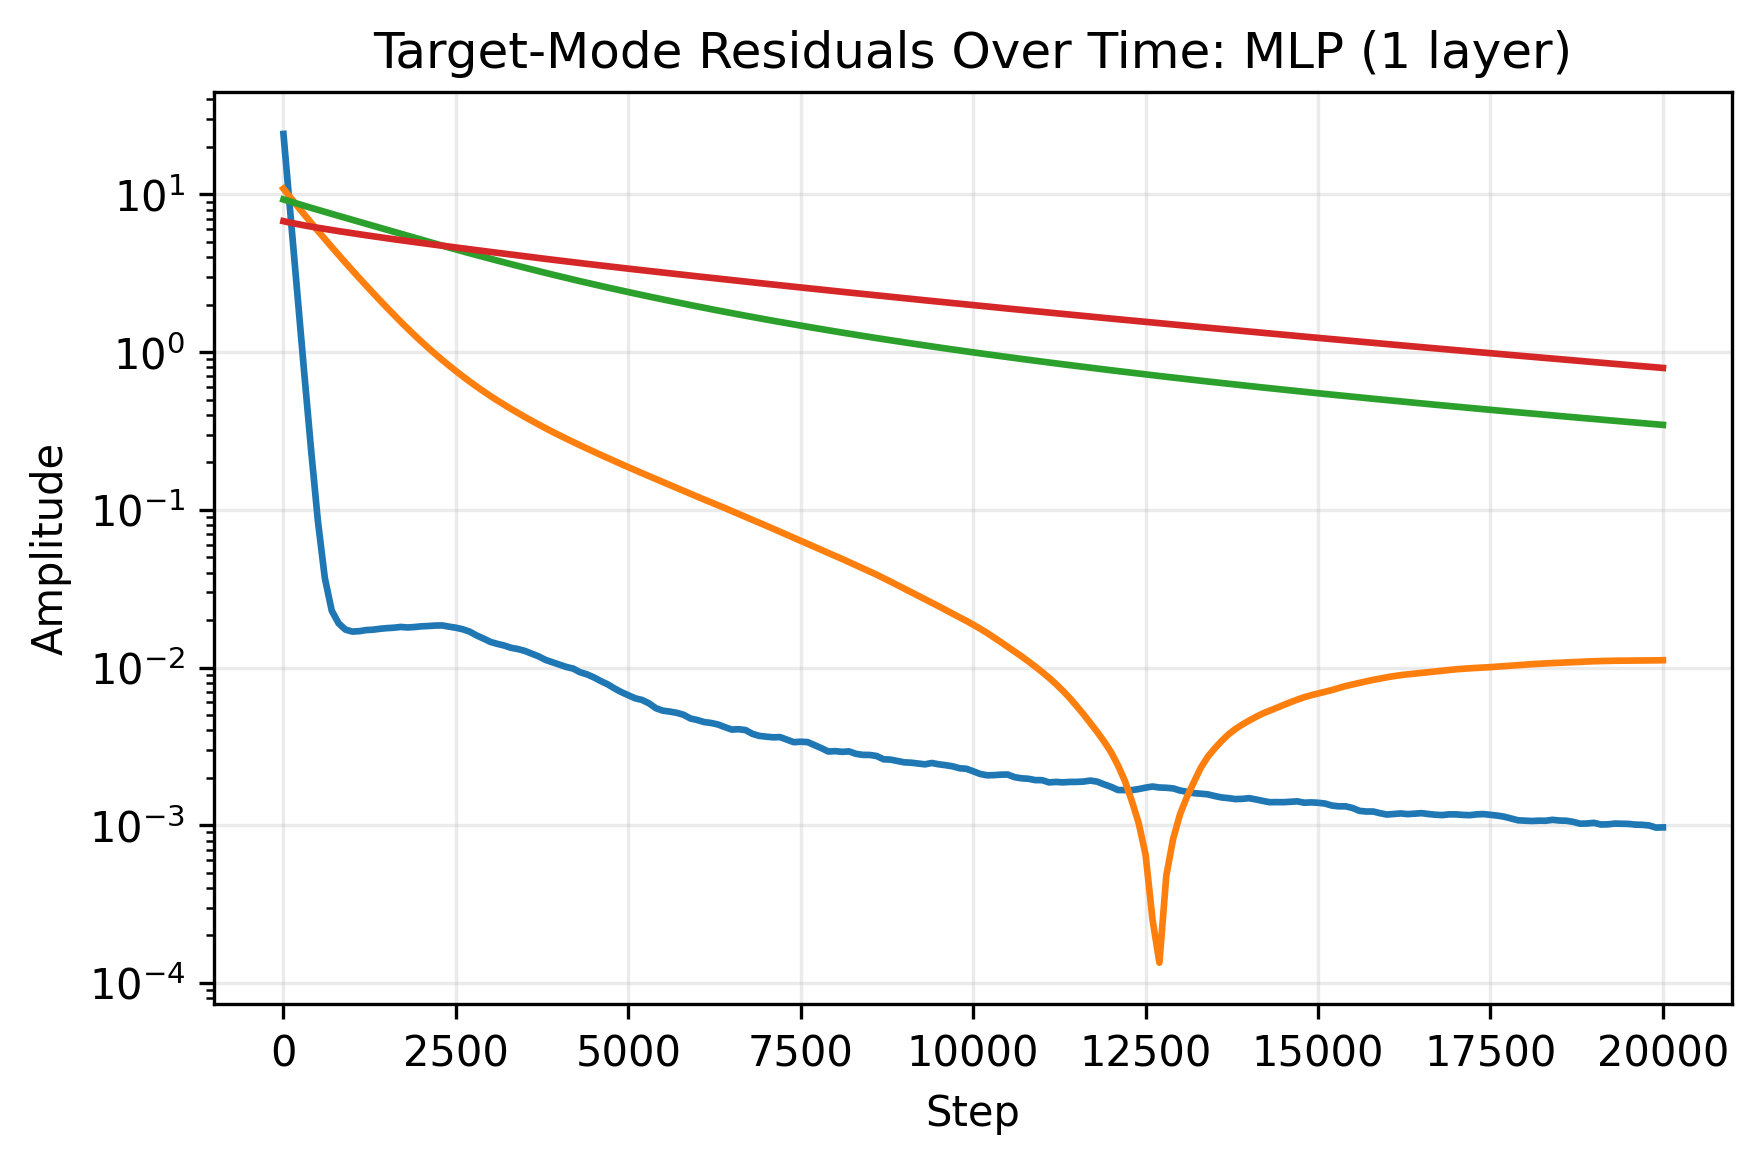
\includegraphics[width=\textwidth]{images/preliminary/mode_residuals_over_time_MLP_(1_layer).png}
		\caption{Single-hidden-layer MLP.}
		\label{fig:prelim-mlp-shallow}
	\end{subfigure}\hfill
	\begin{subfigure}[t]{0.33\textwidth}
		\centering
		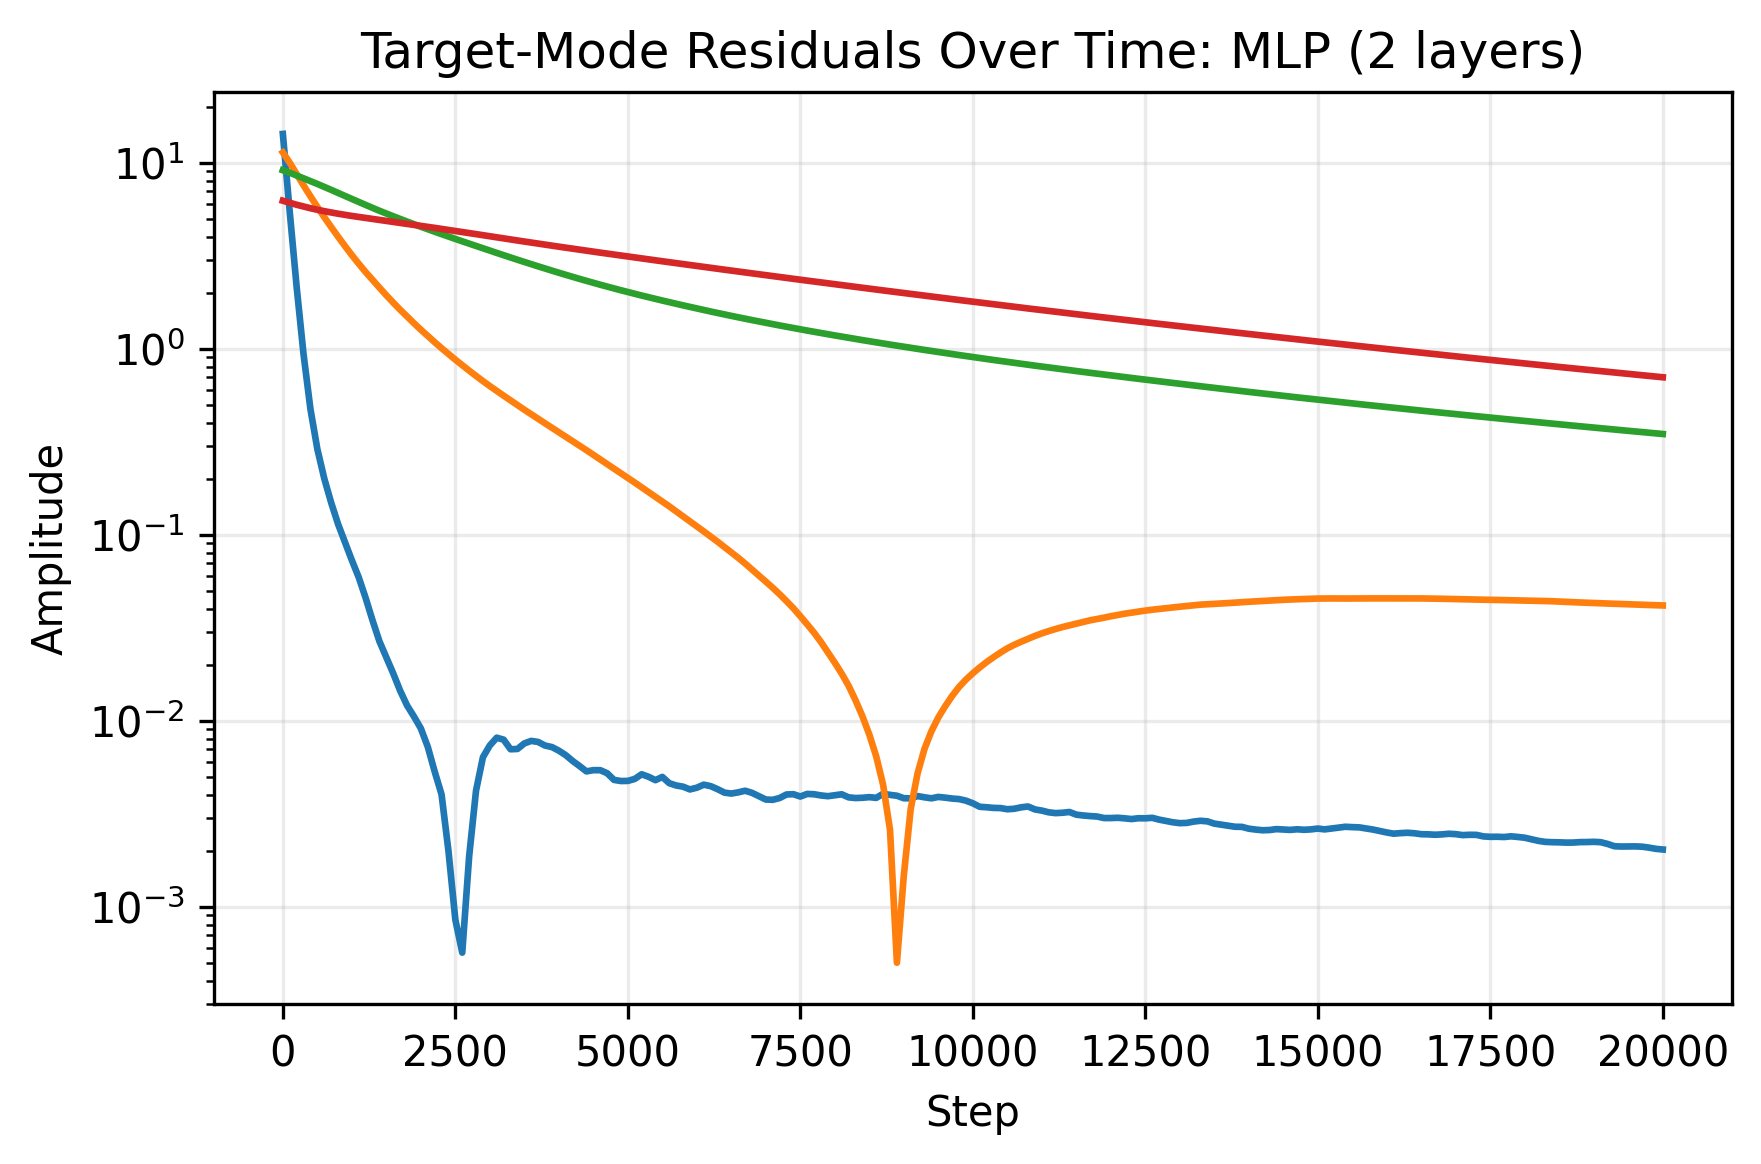
\includegraphics[width=\textwidth]{images/preliminary/mode_residuals_over_time_MLP_(2_layers).png}
		\caption{Two-layer MLP.}
		\label{fig:prelim-mlp-deep}
	\end{subfigure}\hfill
	\begin{subfigure}[t]{0.33\textwidth}
		\centering
		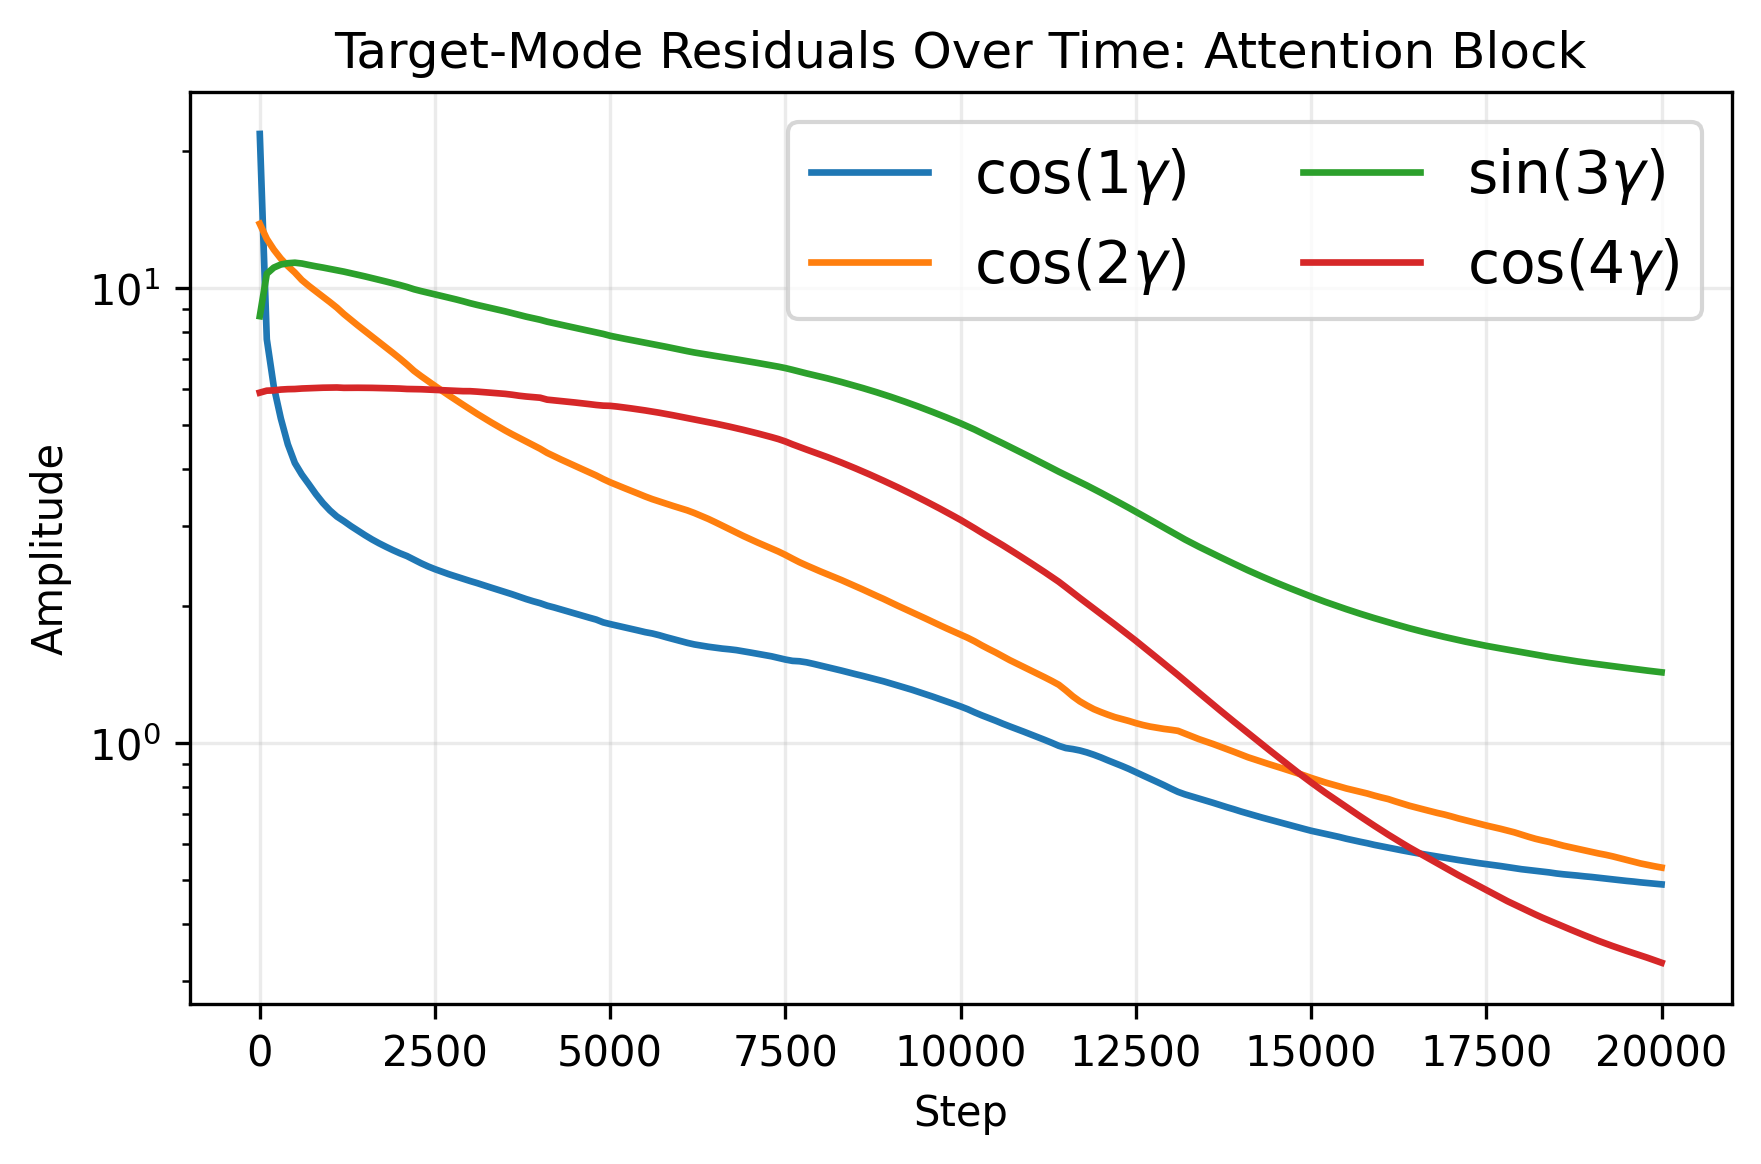
\includegraphics[width=\textwidth]{images/preliminary/mode_residuals_over_time_attention_block.png}
		\caption{Attention block.}
		\label{fig:prelim-attention}
	\end{subfigure}

	\caption{Preliminary experiments across architectures trained at finite width on
		finite data. Each panel shows the residual amplitude of four target modes,
		\(\cos\gamma\), \(\cos 2\gamma\), \(\sin 3\gamma\), and \(\cos 4\gamma\),
		against training step on a logarithmic scale.}
	\label{fig:preliminary-frequency-architectures}
\end{figure}

Figure~\ref{fig:preliminary-frequency-architectures} shows these experiments. In
every case the lowest-frequency mode \(\cos\gamma\) collapses first, within the
first few hundred steps, while the higher-frequency modes decay more slowly, so the
broad low-frequency-first ordering holds across all three architectures. The
ordering is not strict: in the MLPs \(\cos 2\gamma\) overtakes the higher modes and
its coefficient passes through zero, and in the attention block the modes are more
tangled and \(\cos 4\gamma\) eventually decays past the others. Frequency-dependent
learning is therefore not specific to the one-hidden-layer setting, but the precise
spectral picture depends on the operator induced by the architecture, the finite
sample, and the finite-width kernel. This is what motivates the controlled analysis
that follows, where the infinite-width reference operator is explicit and the
effects of finite sampling and finite width can be separated.

\begin{revblock}
	\section{Research gap}\label{sec:research-gap}

	The preceding discussion shows that spectral bias has a clean explanation in
	idealized fixed-kernel settings. In the infinite-width NTK regime, training is
	governed by a fixed operator whose spectrum determines the decay rates of the
	corresponding components of the residual
	\citep{jacot2018ntk,cao2020understandingspectralbiasdeep}. In symmetric
	settings, such as the circle or sphere with the uniform measure, this operator
	can be diagonalized by Fourier or harmonic modes, giving a precise version of
	the ``low frequencies first'' phenomenon
	\citep{basri2019convergence,basri2020frequencybiasneuralnetworks,
		bietti2019inductivebiasneuraltangent}.

	\citet{bowman2022spectralbiasoutsidetraining} prove bounds comparing the
	trajectory of a finite-width network trained on finitely many samples with the
	idealized NTK dynamics obtained at infinite width and infinite data. The
	comparison holds in \(L^2\) over the input distribution and up to a finite time
	horizon, so it describes the learned function away from the training samples as
	well. Their result shows that the network can inherit the bias of the NTK
	integral operator toward its leading eigenfunctions. However, their analysis is
	general as it does not focus on a setting where the eigenfunctions can be written
	explicitly as Fourier modes, nor does it separately track how finite sampling
	and finite width perturb those Fourier eigenspaces.

	This motivates studying a setting where the ideal operator is explicit enough
	that its perturbations can be inspected directly. The circle \(S^1\) with the
	uniform measure provides such a setting. The limiting NTK is a convolution
	operator, the Fourier modes are exact eigendirections, and the corresponding
	eigenvalues can be computed explicitly. This lets us separate the effects that
	are otherwise mixed together: the effect of replacing the continuum measure by
	a finite sample, the effect of replacing the infinite-width kernel by a
	finite-width random kernel, and the effect of allowing the tangent kernel to
	evolve during training.

	What is still missing is therefore a direct account of how the Fourier
	description on \(S^1\) changes under these perturbations.  One would expect the
	low-frequency Fourier structure to persist approximately under finite sampling
	and finite width. In other words, the perturbed eigenvalues should remain close
	to their continuum values, and the eigenspaces of the perturbed operator should
	remain close to the corresponding Fourier frequency subspaces. At the same
	time, these approximations should become more fragile when eigenvalues are
	small, when gaps between eigenvalues are narrow (e.g. in higher frequencies),
	or when the kernel evolves during training.

	\section{Research questions}

	This thesis studies spectral bias on \(S^1\) by comparing the residual dynamics induced by the
	continuum infinite-width NTK operator with those induced by its finite-sample and finite-
	width counterparts.

	Since the full operator acts on an infinite-dimensional function space, we make
	the comparisons on a finite Fourier subspace. For \(K > 0\), let
	\[
		\mathcal H_K
		:=
		\operatorname{span}
		\{1,\sqrt{2}\cos(k\theta),\sqrt{2}\sin(k\theta):1\le k\le K\}.
	\]
	This subspace contains the constant mode and the first \(K\) non-zero Fourier
	frequencies. Working on \(\mathcal H_K\) gives a controlled way to test how far
	the ideal Fourier-mode explanation of spectral bias survives at finite sample
	size and finite width.
\end{revblock}

\paragraph{Main research question.}
To what extent does the spectral decomposition of the continuum infinite-width
NTK operator on \(S^1\) persist on a fixed low-frequency Fourier subspace
\(\mathcal H_K\) under finite-sample and finite-width perturbations?

\paragraph{Subquestions.}
\begin{enumerate}
	\item[(RQ1)] \textbf{Finite-sample perturbation of the continuum operator.}
	      In the infinite-width regime, how does replacing the uniform measure
	      on \(S^1\) by \(n\) i.i.d.\ sampled points affect the action of the
	      continuum NTK operator on the fixed truncated Fourier subspace
	      \(\mathcal H_K\)?
	      More precisely, how close is the sampled operator to the diagonal
	      Fourier prediction on this subspace, and what are the consequences
	      for the associated residual dynamics?
	\item[(RQ2)] \textbf{Finite-width perturbation in the continuum setting.}
	      With the continuum measure on \(S^1\) kept fixed, how does finite
	      network width affect the tangent-kernel dynamics on the fixed truncated
	      Fourier subspace \(\mathcal H_K\), both at initialization and during
	      training?
	      More precisely, how close is the finite-width tangent kernel at
	      initialization to the infinite-width tangent kernel, and how does
	      the evolution of this tangent kernel during training change the decay of Fourier
	      modes, their alignment, and their effective learning rates?
\end{enumerate}

\section{Contributions}
\label{sec:contributions}

\begin{itemize}
	\item We derive the infinite-width reference model for the specific network
	      studied in this thesis. Closely related two-layer analyses often
	      simplify the NTK by training only the first-layer weights and biases
	      while keeping the output weights fixed
	      \citep{basri2019convergence,basri2020frequencybiasneuralnetworks}.
	      Here, we keep the output weights trainable and include their
	      contribution to the NTK. This gives an explicit kernel on \(S^1\),
	      explicit Fourier learning rates, and the baseline used in the rest of
	      the thesis.

	\item We study how this Fourier-frequency picture changes when the continuum
	      input distribution is replaced by finitely many sampled points. For a
	      fixed low-frequency subspace, we prove non-asymptotic bounds showing
	      that the sampled Fourier structure remains close to the idealized
	      continuum prediction when the sample size is large enough.

	\item We support the finite-sample analysis with numerical experiments. These
	      experiments compare the predicted frequency-wise learning rates with
	      the rates observed on sampled data, and show that the agreement improves
	      as the number of samples increases.

	\item We study the effect of finite network width when the tangent kernel is
	      frozen at initialization. On the same low-frequency subspace, we prove
	      that the finite-width operator concentrates around the infinite-width
	      prediction as width increases, and we verify this numerically using
	      eigenspace-alignment diagnostics.

	\item We empirically study the evolving finite-width tangent kernel during
	      training. We compare frozen and evolving dynamics across widths, and track
	      mode-wise residual decay, Fourier-subspace alignment, effective decay-rates,
	      and kernel drift. The experiments suggest that kernel evolution
	      helps at small width mainly by increasing low-frequency spectral
	      strength, even though it can move some eigenspaces away from the Fourier
	      reference. This advantage becomes smaller as width increases.
\end{itemize}

Together, these results show how the clean Fourier description from the
infinite-width model changes when we move to finite data and finite network
width. For finite sampling and frozen finite width, we give explicit
non-asymptotic bounds. For the evolving finite-width kernel during training, we
provide an empirical analysis showing how kernel evolution changes residual
decay, Fourier alignment, and spectral strength. Developing comparable theory
for this evolving-kernel regime remains the main open direction.
